% fig_enhancement_budget.tex - Enhancement factor breakdown (waterfall chart)
% Standalone compilation: pdflatex fig_enhancement_budget.tex
\documentclass[tikz,border=5pt]{standalone}
\usepackage{pgfplots}
\usepackage{amsmath}
\pgfplotsset{compat=1.18}

\begin{document}
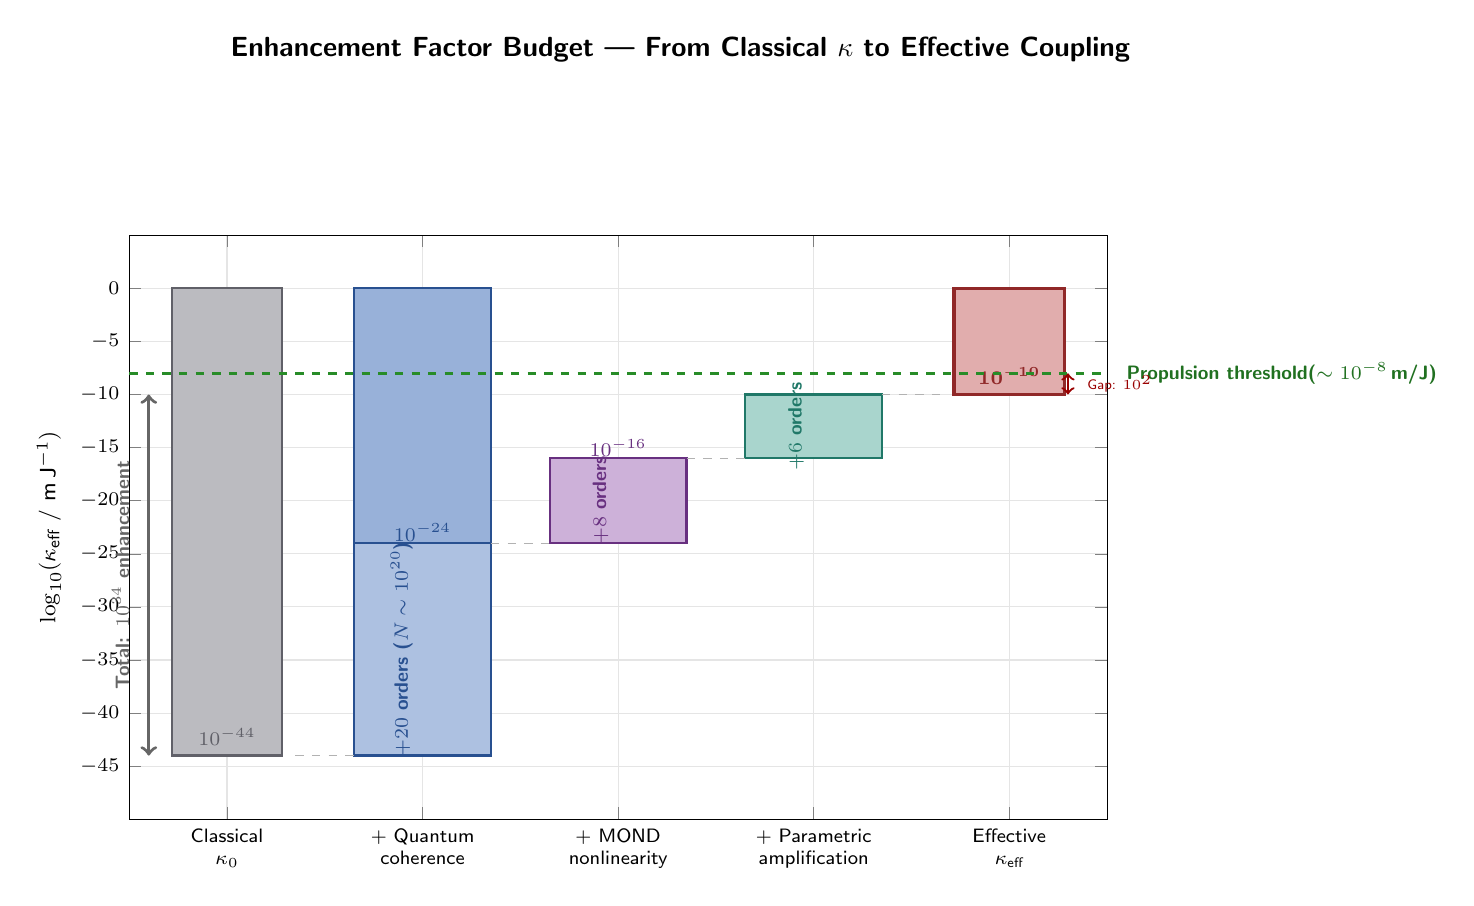
\begin{tikzpicture}

\definecolor{classicalGray}{RGB}{120,120,130}
\definecolor{qcBlue}{RGB}{50,100,180}
\definecolor{mondPurple}{RGB}{130,60,160}
\definecolor{paramTeal}{RGB}{40,150,130}
\definecolor{finalRed}{RGB}{180,50,50}
\definecolor{threshGreen}{RGB}{40,140,40}

% ============================================================
% WATERFALL CHART
% ============================================================
\begin{axis}[
    width=14cm, height=9cm,
    ymin=-50, ymax=5,
    xmin=-0.5, xmax=4.5,
    ylabel={$\log_{10}(\kappa_\text{eff}$ / m\,J$^{-1})$},
    ylabel style={font=\footnotesize\sffamily},
    xlabel style={font=\footnotesize\sffamily},
    tick label style={font=\scriptsize\sffamily},
    xtick={0,1,2,3,4},
    xticklabels={
        {Classical\\$\kappa_0$},
        {+ Quantum\\coherence},
        {+ MOND\\nonlinearity},
        {+ Parametric\\amplification},
        {Effective\\$\kappa_\text{eff}$}
    },
    x tick label style={font=\scriptsize\sffamily, align=center, text width=2.5cm},
    grid=major,
    grid style={black!10},
    ytick={-45,-40,-35,-30,-25,-20,-15,-10,-5,0},
    clip=false,
]

% --- Classical baseline bar ---
\addplot[ybar, bar width=40pt, fill=classicalGray!50, draw=classicalGray!80!black, thick]
    coordinates {(0,-44)};

% --- Quantum coherence increment ---
% Floating bar from -44 to -24
\addplot[ybar interval, fill=qcBlue!50, draw=qcBlue!80!black, thick]
    coordinates {(0.65,-44) (1.35,-44)};  % dummy
\fill[qcBlue!40] (axis cs:0.65,-44) rectangle (axis cs:1.35,-24);
\draw[qcBlue!80!black, thick] (axis cs:0.65,-44) rectangle (axis cs:1.35,-24);

% --- MOND nonlinearity increment ---
% Floating bar from -24 to -16
\fill[mondPurple!40] (axis cs:1.65,-24) rectangle (axis cs:2.35,-16);
\draw[mondPurple!80!black, thick] (axis cs:1.65,-24) rectangle (axis cs:2.35,-16);

% --- Parametric amplification increment ---
% Floating bar from -16 to -10
\fill[paramTeal!40] (axis cs:2.65,-16) rectangle (axis cs:3.35,-10);
\draw[paramTeal!80!black, thick] (axis cs:2.65,-16) rectangle (axis cs:3.35,-10);

% --- Final effective coupling bar ---
\addplot[ybar, bar width=40pt, fill=finalRed!40, draw=finalRed!80!black, very thick]
    coordinates {(4,-10)};

% --- Connector lines (dashed) ---
\draw[black!30, dashed, thin] (axis cs:0.35,-44) -- (axis cs:0.65,-44);
\draw[black!30, dashed, thin] (axis cs:1.35,-24) -- (axis cs:1.65,-24);
\draw[black!30, dashed, thin] (axis cs:2.35,-16) -- (axis cs:2.65,-16);
\draw[black!30, dashed, thin] (axis cs:3.35,-10) -- (axis cs:3.65,-10);

% --- Enhancement factor labels ---
\node[font=\scriptsize\sffamily\bfseries, qcBlue!80!black, rotate=90, anchor=south]
    at (axis cs:1,-34) {$+20$ orders ($N \sim 10^{20}$)};
\node[font=\scriptsize\sffamily\bfseries, mondPurple!80!black, rotate=90, anchor=south]
    at (axis cs:2,-20) {$+8$ orders};
\node[font=\scriptsize\sffamily\bfseries, paramTeal!80!black, rotate=90, anchor=south]
    at (axis cs:3,-13) {$+6$ orders};

% --- Value labels on bars ---
\node[font=\scriptsize\sffamily, classicalGray!80!black, above]
    at (axis cs:0,-44) {$10^{-44}$};
\node[font=\scriptsize\sffamily, qcBlue!80!black]
    at (axis cs:1,-23) {$10^{-24}$};
\node[font=\scriptsize\sffamily, mondPurple!80!black]
    at (axis cs:2,-15) {$10^{-16}$};
\node[font=\scriptsize\sffamily\bfseries, finalRed!80!black, above]
    at (axis cs:4,-10) {$\mathbf{10^{-10}}$};

% --- Propulsion threshold line ---
\draw[threshGreen, very thick, dashed]
    (axis cs:-0.5,-8) -- (axis cs:4.5,-8);
\node[font=\scriptsize\sffamily\bfseries, threshGreen!80!black, anchor=west]
    at (axis cs:4.55,-8) {Propulsion threshold\\($\sim 10^{-8}$\,m/J)};

% --- Annotation: gap remaining ---
\draw[<->, red!60!black, thick]
    (axis cs:4.3,-10) -- (axis cs:4.3,-8);
\node[font=\tiny\sffamily, red!60!black, right]
    at (axis cs:4.35,-9) {Gap: $10^2$};

% --- Arrow showing total enhancement ---
\draw[<->, black!60, very thick]
    (axis cs:-0.4,-44) -- (axis cs:-0.4,-10);
\node[font=\scriptsize\sffamily\bfseries, black!60, rotate=90, anchor=south]
    at (axis cs:-0.45,-27) {Total: $10^{34}$ enhancement};

\end{axis}

% ============================================================
% TITLE
% ============================================================
\node[font=\normalsize\sffamily\bfseries, anchor=south] at (7,9.5)
    {Enhancement Factor Budget --- From Classical $\kappa$ to Effective Coupling};

\end{tikzpicture}
\end{document}
